%!TEX root = ../main.tex

Μια μικρή περιγραφή των κεφαλαίων

\section{Visual Impairment}
Διάφορα είδη προβλημάτων όρασης\\
Δυσκολίες και τρέχουσες λύσεις

\section{AR, VR and XR}
Ορισμός\\
Τρέχουσες χρήσεις\\
Συσκευές που παρέχουν αυτές τις δυνατότητες

\section{Hololens}
Hololens\\
Hololens features\\
Description of the device\\
Τρόποι αλληλεπίδρασης\\
Spatial Mapping (Υπολογιστική όραση) and Spatial Audio

\section{Εργαλεία ανάπτυξης για Hololens}

\subsection{Unity}
Περιγραφή περιβάλλοντος

\subsection{Microsoft Visual Studio}
Μικρή περιγραφή της χρήσης του

\subsection{Mixed Reality Toolkit}

% \begin{figure}
%   \centering
%   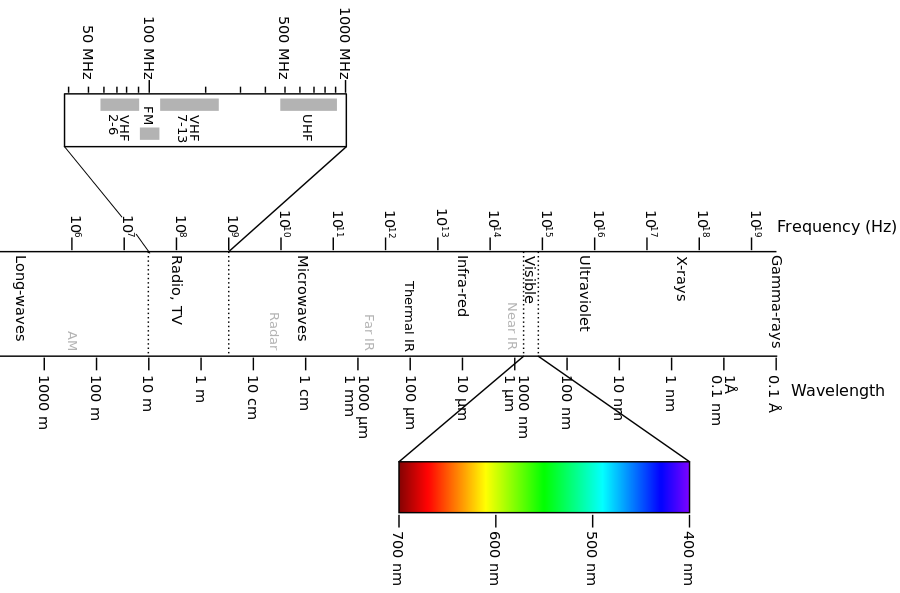
\includegraphics[width=\textwidth]{spectrum}
%   \caption{Το φάσμα της Ηλεκτρομαγνητικής Ακτινοβολίας}
%   \label{fig:spectrum}
% \end{figure}